%\documentclass{beamer}
\documentclass[hyperref={pagelabel=false,colorlinks=true,linkcolor=blue,citecolor=blue},12pt]{beamer}
\usepackage[T1]{fontenc}
\usepackage[latin1]{inputenc}
\usepackage{amsmath}
\usepackage{algorithm}
\usepackage{algorithmic}

\usetheme{Warsaw}

\title[Learning Music Representation using Recurrent Neural Networks]{Learning Music Representation using Recurrent Neural Networks}
\author{Cl�ment Jambou}
\institute{Imperial College of London, Departement of Computing}
\date{8 September 2014}


\begin{document}


\AtBeginSection[]
{
  \begin{frame}
  \tableofcontents[currentsection]
  \end{frame} 
}


\begin{frame}
\titlepage
\end{frame}


\begin{frame}
\tableofcontents

\end{frame}


\section{State of the art and Motivation}

    \subsection{ State of the Art}

\begin{frame}
    \frametitle{Neural networks}

    \begin{itemize} 
        \item Feed Forward (FFNN)
        \item Recurrent (RNN)
    \end{itemize}
    \begin{center}
        \begin{figure}
            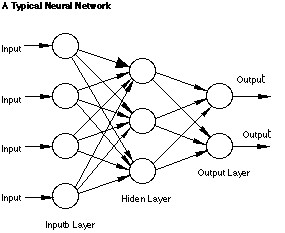
\includegraphics[width=0.3\textwidth]{Figures/network.jpeg} 
            \hspace{1cm} 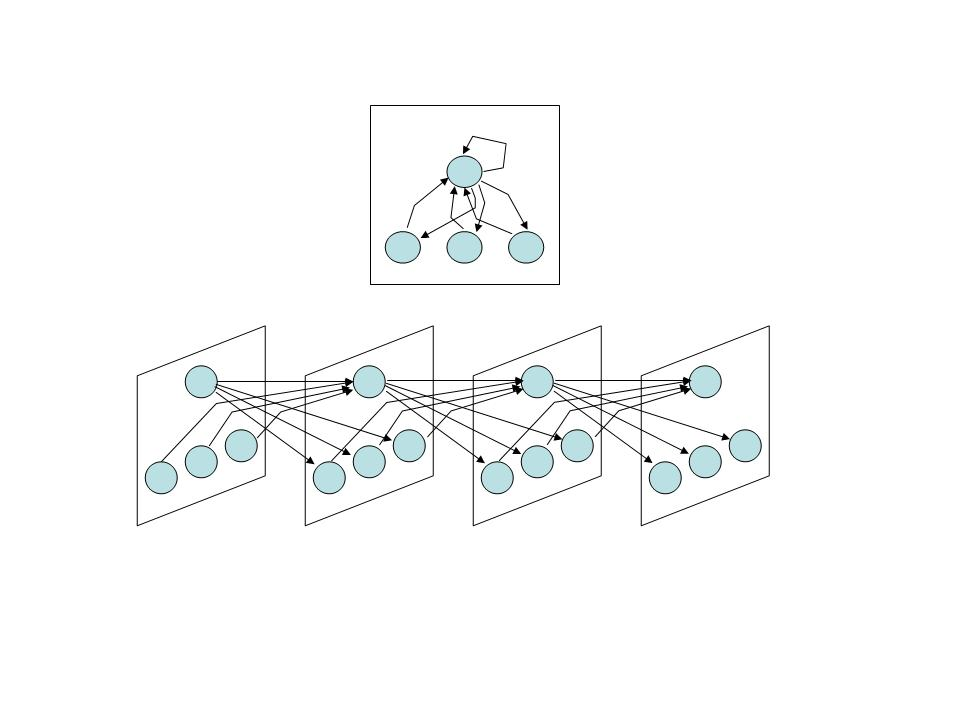
\includegraphics[width=0.5\textwidth]{Figures/rnn.png} 
        \end{figure}
    \end{center}

\end{frame}

\begin{frame}
    \frametitle{model of RNN}
    Given a sequence of inputs: $x_1, x_2, ... x_t$ and the hidden states $h_1, h_2, ..., h_t$.
    $$
    \begin{array}{rcr} 
        h_0 & = & a(W_{hx}  * x_0 + b_{init} + b_h)  \\ 
        h_i & = & a(W_{hx}  * x_i + W _{hh} * h_{i-1} + b_h)  \\ 
        \hat{y}_i & = & a'(W_{yh} + b_y)

    \end{array}
    $$

\end{frame}


\begin{frame}
    \frametitle{Training : Backpropagation}
    Backpropagation = Gradient descent on loss. 

    \begin{itemize} 
        \item use of the derivative of composition product to go back layer after layer...
        \item backpropagation through time for RNNs
    \end{itemize}
    \begin{center}
        \begin{figure}
            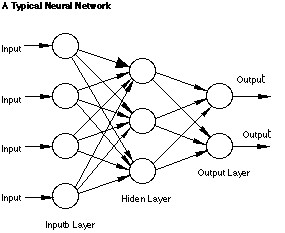
\includegraphics[width=0.4\textwidth]{Figures/network.jpeg} 
        \end{figure}
    \end{center}

\end{frame}


\begin{frame}
    \frametitle{Vanishing gradient and Hessian Free Optimization}

    \begin{itemize} 
        \item Deep $\Rightarrow$ vanishing gradient (one more layer = one more Matrix multiplication)
        \item RNN : as deep as the number of timesteps. 
    \end{itemize}
    \begin{center}
        \begin{figure}
            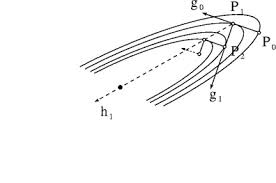
\includegraphics[width=0.3\textwidth]{Figures/gradient_ellipse.jpg} 
        \end{figure}
    \end{center}

    Solution : Use second order information.
    Hessian Free Optimization use a quadratic approximation of the fitness function and performs the first steps of conjuguate gradient descent.

\end{frame}

\subsection{Motivation}

\begin{frame}
	\frametitle{Motivation:}
    \begin{itemize}
        \item Growth of computational power led to think : "The bigger network, the better."
        \item Current RNN structure uses dense Matrix where the brain connections map is sparse. 
        \item Long Short-Term Memory Networks (LSTM) proposed a specific change in the RNN architecture. 
    \end{itemize}
    
    \begin{itemize}

     \item Number of Neurons in human brain : $\sim 10^{11}$ 
     \item Number of Synapse in human brain : $\sim 10^{14}, 10 ^{15}$ 
    \end{itemize}
\end{frame}

\section{Study of RNNs}

 
\begin{frame}
    \frametitle{Experiment:}
    Pretrained RNN on a memory problem: 100 timesteps long sequences of bits. 
    \newline
    Loss: Cross correlation of the output of the last timestep and the first input (Remember the first input)
    \begin{center}
         \begin{figure}
             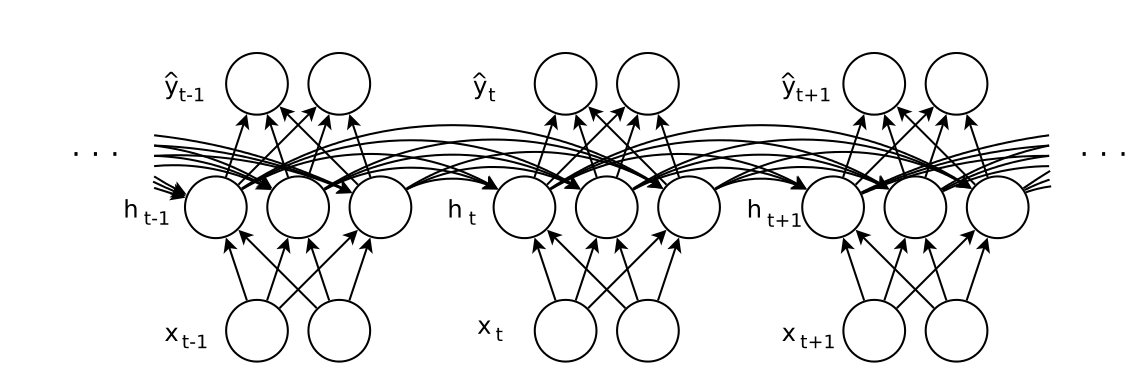
\includegraphics[width=0.5\textwidth]{Figures/RNN.png}
        \end{figure}
    \end{center}
    Training : 8 hours, with Hessian Free Optimization

\end{frame}

  
\begin{frame}
    \frametitle{Plotting}
   Goal : Find a way of plotting the RNN.
    \begin{itemize}
        \item use weights as spring.
        \item spectral analysis of Laplacian matrix.
    \end{itemize}
    \begin{center}
         \begin{figure}
            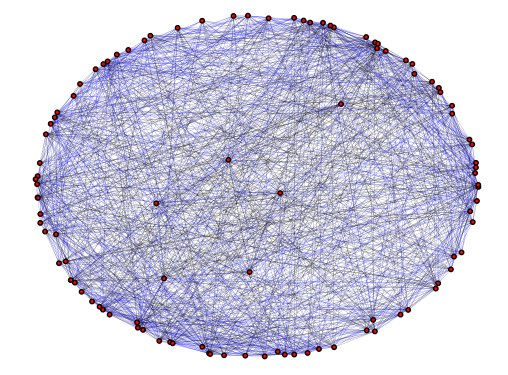
\includegraphics[width=0.3\textwidth]{Figures/weighted_graph_spring.png} 
            \hspace{1cm} 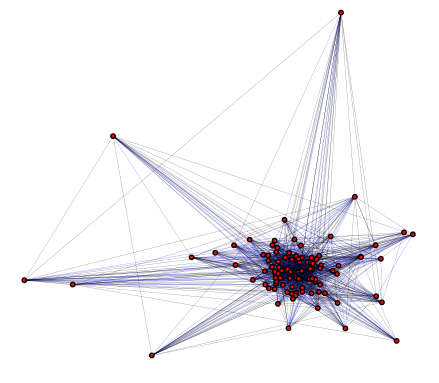
\includegraphics[width=0.3\textwidth]{Figures/weighted_graph_spectral.png} 
        \end{figure}
    \end{center}

\end{frame}

\begin{frame}
    \frametitle{Question : Are all the neurons useful?}
    We remove one neuron at a time (by replacing its input/output weights in Whh with 0) and test the network on a dataset. 
    \begin{center}
         \begin{figure}
            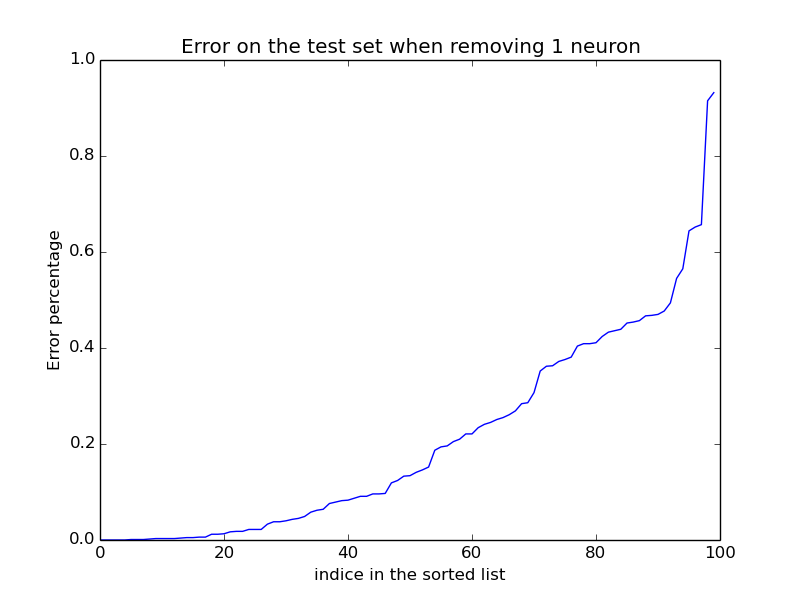
\includegraphics[width=0.45\textwidth]{Figures/error_test_set_remove_neuron.png} 
        \end{figure}
    \end{center}
    Results : Neurons importance is very unequal (though the sum of absolute value of the weights is very constrained) 
    We order the neurons using this method to obtain the "worth" of a neuron.
\end{frame}


\begin{frame}
    \frametitle{Comparaison with classical metrics}
    We compare the "worth" with different metrics
    
    \begin{itemize}
        \item M1 : The sum of the absolute value of the in and out weights on the hidden-to-hidden connections
        \item M2 : The sum of the in and out weights on the hidden-to-hidden connections
        \item M3 : The absolute value of the sum of the in and out weights on the hidden-to-hidden connections
        \item M4 : The clustering index
        \item M5 : The absolute value of the ouput weights ( of the hidden to output matrix) 
        \item M6 : The absolute value of the input weights ( of the input to hidden matrix) 
        \item M7 : The sum of the two previous metrics.
    \end{itemize}

\end{frame}


\begin{frame}
    \frametitle{Comparaison with classical metrics}
    \begin{center}
         \begin{figure}
            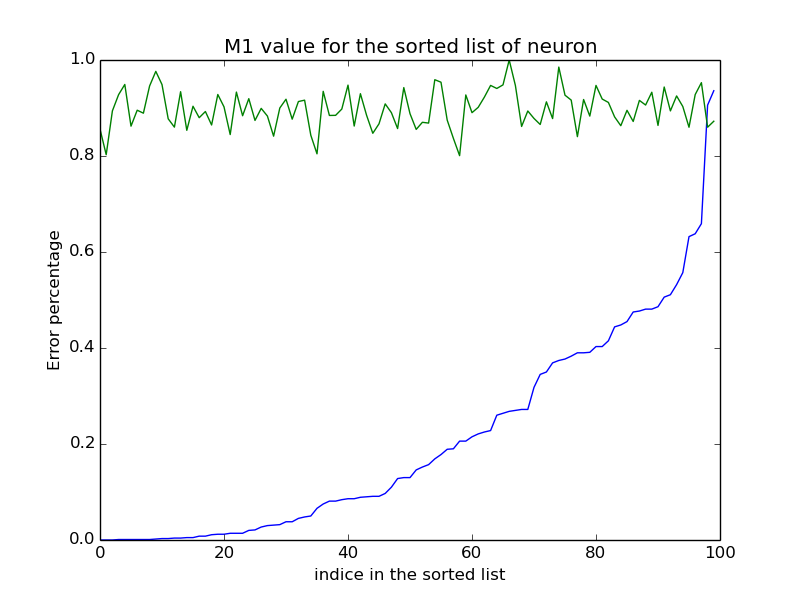
\includegraphics[width=0.25\textwidth]{Figures/m1.png}
            \hspace{0.1cm} 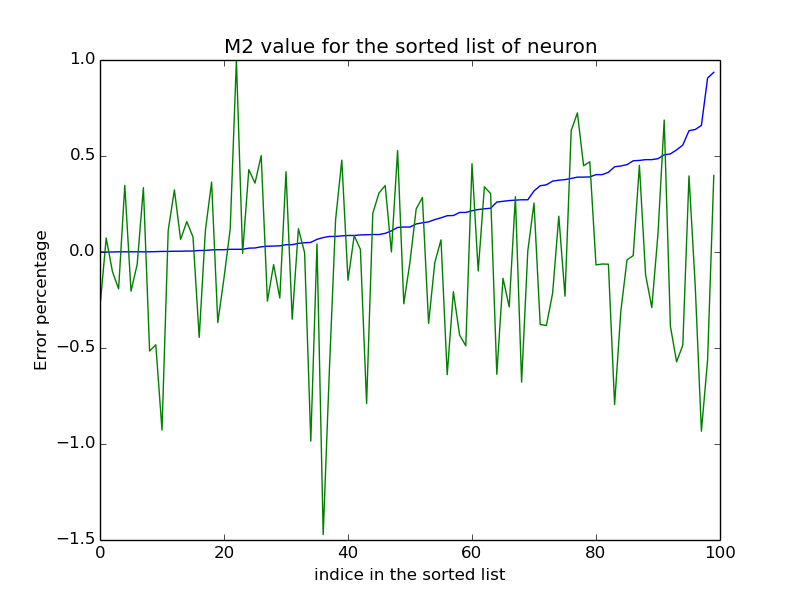
\includegraphics[width=0.25\textwidth]{Figures/m2.png}
            \hspace{0.1cm} 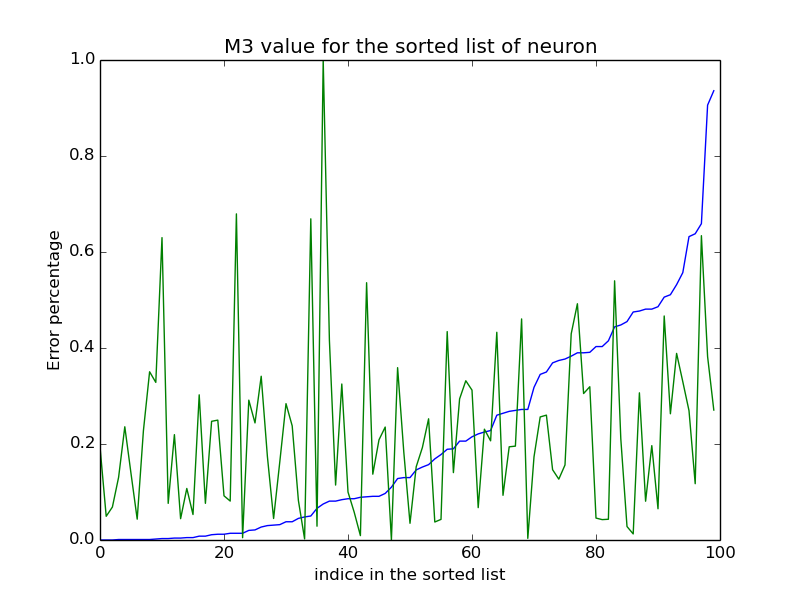
\includegraphics[width=0.25\textwidth]{Figures/m3.png}
            \hspace{0.1cm} 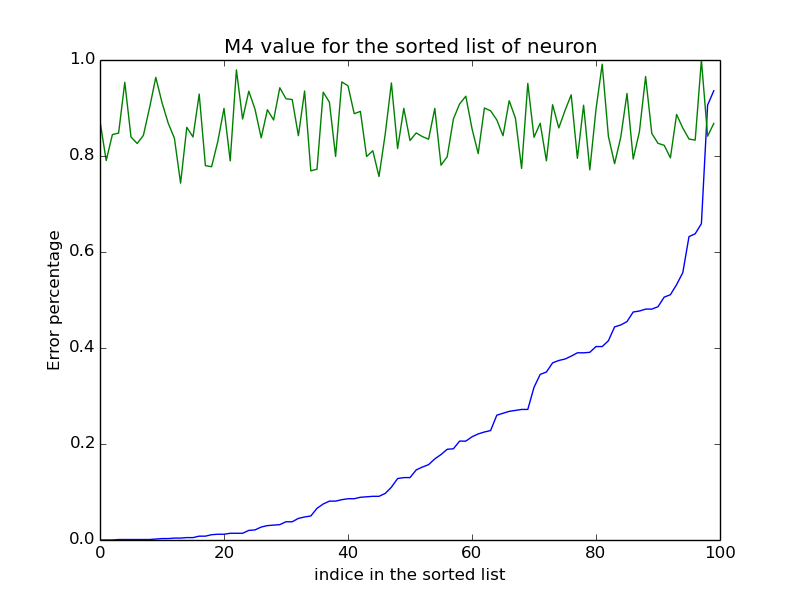
\includegraphics[width=0.25\textwidth]{Figures/m4.png}
        \end{figure}
        \begin{figure}
            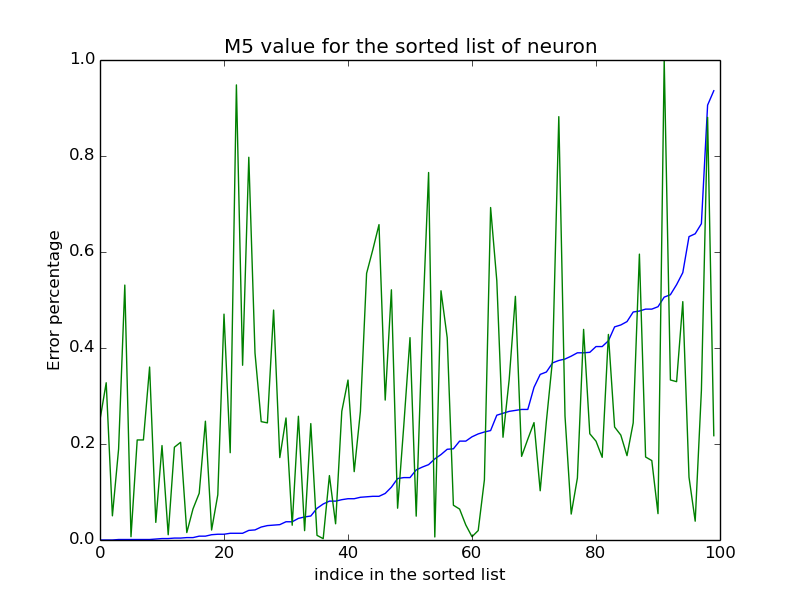
\includegraphics[width=0.25\textwidth]{Figures/m5.png}
            \hspace{1cm} 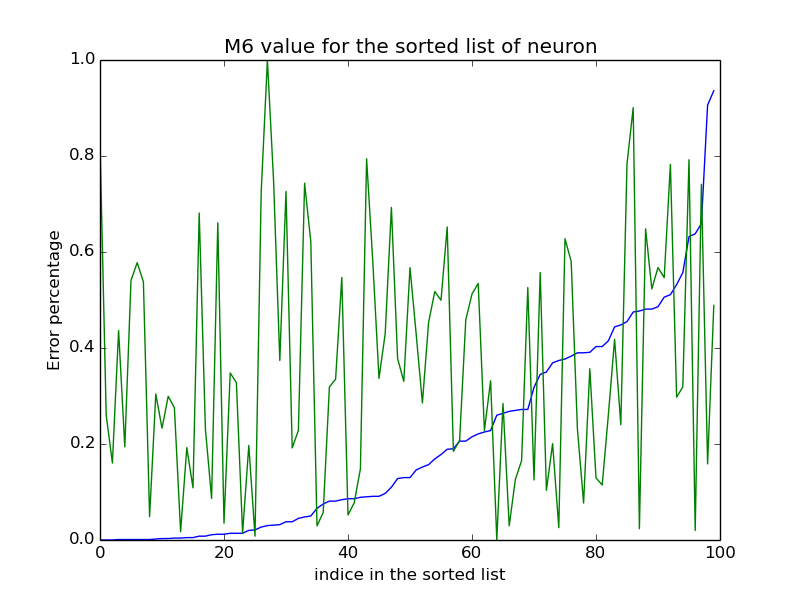
\includegraphics[width=0.25\textwidth]{Figures/m6.png}
            \hspace{1cm} 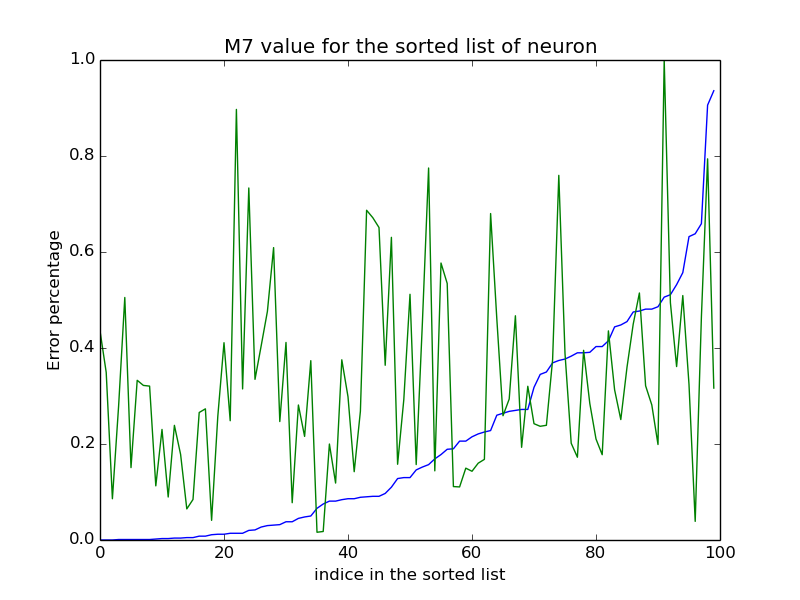
\includegraphics[width=0.25\textwidth]{Figures/m7.png}
        \end{figure}
    \end{center}

\end{frame}


\begin{frame}
    \frametitle{Comparaison with classical metrics}

\begin{figure}[!htb]
    \centering
    \begin{tabular}{|l|l|}
        \hline
        M1 & 3118 \\ \hline
        M2 & 3294 \\ \hline
        M3 & 3512 \\ \hline
        M4 & 3388 \\ \hline
        M5 & 3244 \\ \hline
        M6 & \textbf{2944} \\ \hline
        M7 & 3402 \\
        \hline
    \end{tabular}
    \label{fig:metrics}
    \rule{35em}{0.5pt}
    \caption[Table presenting the value of d for the different metrics ]{Table presenting the value of d for the different metrics}
\end{figure}

Results: None of the natural metrics have satisfying results which proves that the dynamic within a RNN is not well understood.

\end{frame}


\begin{frame}
    \frametitle{Compairing the connections}
    We perform the same experiment on each connection
    \begin{center}
        \begin{figure}
            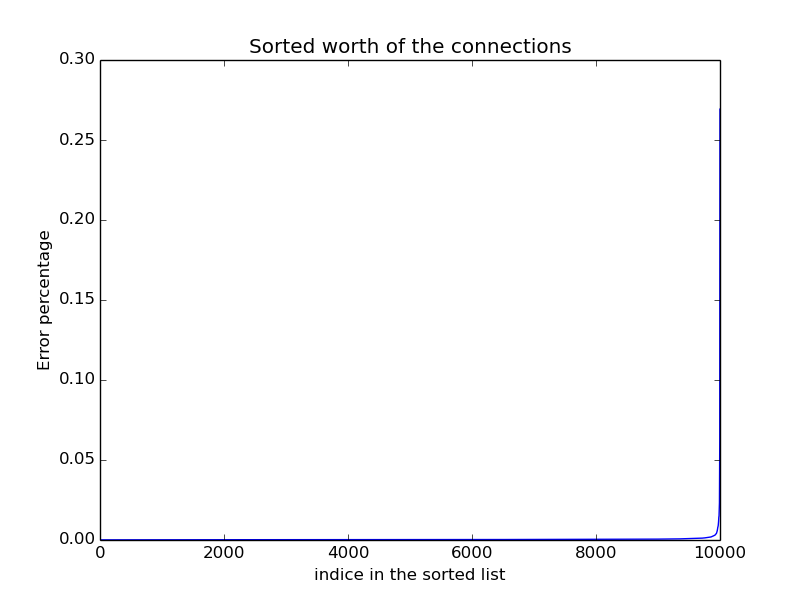
\includegraphics[width=0.5\textwidth]{Figures/score_worth_connection.png} 
        \end{figure}
    \end{center}
    Result : Many connections could be removed without influencing the results of the network -> confirm the intuition of using sparse matrix.

\end{frame}

\begin{frame}
    \frametitle{Correlation between the weight and "worth" of a connection}
    We sort the connections based on the absolute value of the weight and display in blue their "worth" based on the previous experiment.
    \begin{center}
        \begin{figure}
            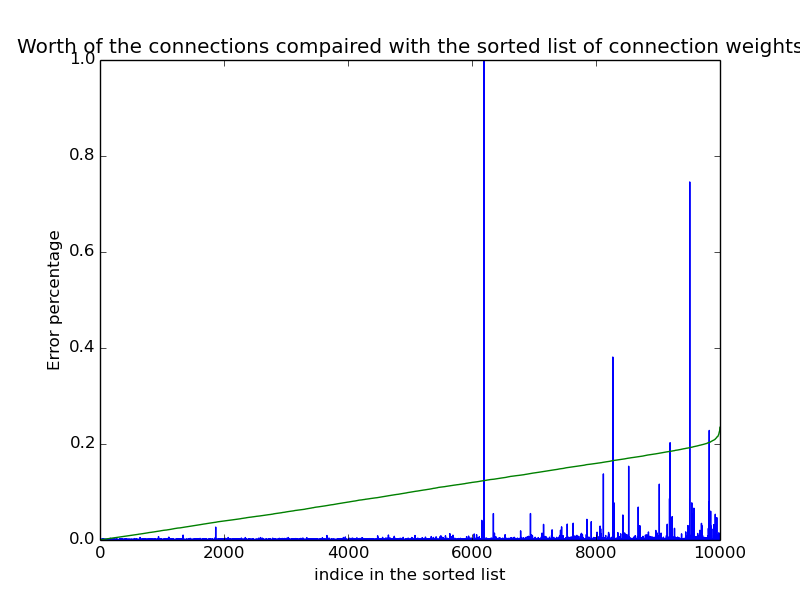
\includegraphics[width=0.4\textwidth]{Figures/score_vs_weight_connections.png} 
        \end{figure}
    \end{center}
    Result: having a large weight, even if it is a necessary condition does not mean that the connection is important. 

\end{frame}

   

\section{Self Growing Recurrent Neural Networks (SGRNN)}
 
\begin{frame}
    \frametitle{Goals}
    \begin{itemize}
          \item Use the previous experiments and results to build a new learning algorithm
          \item Propose smooth modification of the architecture.
    \end{itemize}

    In this Section, we introduce Self-Growing Recurrent Neural Network (SGRNN), which is a Recurrent Neural Network that change its architecture as well as its weights during learning.

\end{frame}


\begin{frame}
    \frametitle{Learning algorithm}
    \begin{algorithm}[H]
        \caption{Learning algorithm}
        \begin{algorithmic}
        \STATE $ weightsInit() $
        \WHILE{$continueTraining$}
            \FOR{$i \in [1: K]$}
                \STATE $HFOStep()$
            \ENDFOR
            \STATE $evolutionStep()$
        \ENDWHILE
        
        \end{algorithmic}
    \end{algorithm}
    The evolution step is : 
    \begin{itemize}
        \item Selection
        \item Cross-Over.
    \end{itemize}
\end{frame}

\begin{frame}
    \frametitle{Preliminary computation and Selection}
        \begin{itemize}
            \item Before performing the selection and cross-over, we order the neurons based on their worth on a valid set ( as in the previous chapter)
            \item During the selection we remove the first $k$ percent of the neurons  
        \end{itemize}

\end{frame}


\begin{frame}[fragile]
    \frametitle{Cloning a neuron}
     $$
    \begin{array}{rcr} 
        h_0 & = & a(W_{hx}  * x_0 + b_{init} + b_h)  \\ 
        h_i & = & a(W_{hx}  * x_i + W _{hh} * h_{i-1} + b_h)  \\ 
        \hat{y}_i & = & a'(W_{yh} + b_y)

    \end{array}
    $$
    
    The new cloned neuron has the same state.
\end{frame}


\begin{frame}[fragile]
    \frametitle{Cloning a neuron}
 
    \small\begin{verbatim}
def insert_in_model(self, i):
    #clone neurons i
    self.whh = np.array(np.hstack([self.whh, 
        np.matrix(self.noise(self.whh[:, i])).T])) 
    self.whh[i] = 0.5 * self.whh[i]  
    self.whh = np.vstack([self.whh, 
        self.noise(self.whh[i])])
    self.Wx = np.array(np.hstack([self.Wx, 
        np.matrix(self.Wx[:, i]).T])) 
    self.bh = np.hstack([self.bh, self.bh[i]]) 
    self.h0 = np.hstack([self.h0, self.h0[i]])
    self.Wy[:, i] = 0.5 * self.Wy[:, i]  
    self.Wy = np.array(np.vstack([self.Wy, self.Wy[i]])) 
    \end{verbatim}

\end{frame}

\begin{frame}[fragile]
    \frametitle{Cross-over (Repopulation)}
        \begin{itemize}
            \item We clone the last $k$ percent of the neurons  
        \end{itemize}

    \begin{verbatim}

    def noise(self, vector):
        cov = 0.01 * np.diag(np.abs(vector))
        res = np.random.multivariate_normal(vector,
        cov)
        return res.astype(theano.config.floatX)
    \end{verbatim}
    
    We introduce noise so the parameters are different. Because HFO can make sense of small differences between parameters gradient.

\end{frame}

\section{Application on a natural problem : Music Generation}


\begin{frame}
    \frametitle{Music Data}
    
       To train the network we use a dataset of MIDI files from Chorales of J.S Bach
       \begin{itemize}
           \item We take samples of 10 timesteps long sequences of chords.
           \item one bit for each note: 1 $\Rightarrow$ note is playing 0, $ \Rightarrow$ note is not playing
           \item The network is trained to predict the bit vector for the next timestep
       \end{itemize}
\end{frame}


\begin{frame}
    \frametitle{Result and demo}
    We compare the learning curves of classical RNN with fixed number of neurons (20 (green and 50 (red)) and the SGRNN (blue)
        \begin{figure}
            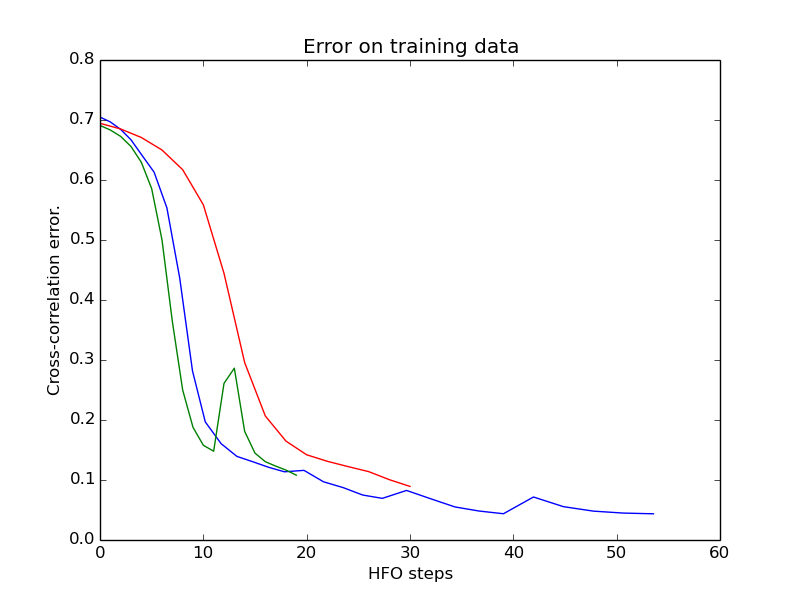
\includegraphics[width=0.6\textwidth]{Figures/sgrnn_training.png} 
        \end{figure}   
\end{frame}


\begin{frame}
    \frametitle{Result and demo}
 
    Demo : We use the network to recursively predict the next timestep. 
    \begin{itemize}
        \item sample before training
        \item sample after training
    \end{itemize}
\end{frame}

\begin{frame}
    \begin{center}
    Thank you
    \begin{figure}
            
\includegraphics[width=0.1\textwidth]{Figures/Logo.jpg} 
        \end{figure}   
    \end{center}
\end{frame}

%\frame[shrink=30] 
%{ 
%    \frametitle{References} 
%    \bibliographystyle{alpha} 
%    \bibliography{Bibliography.bib} 
%}

\end{document}
